\documentclass[a4paper,10pt]{book}

\usepackage{graphicx}
\usepackage[pdftex,bookmarks=true,breaklinks=true,colorlinks,linkcolor=black,filecolor=blue,urlcolor=blue,hypertexnames=false]{hyperref}

\hypersetup{
pdfauthor = {Nathan Dumont},
pdftitle = {Z80 Project Mark 2: Documentation},
pdfsubject = {System Manual}}

\usepackage{fancyhdr}
\pagestyle{fancy}
\renewcommand{\chaptermark}[1]{\markboth{#1}{}}
\fancyhead{}
\fancyhead[R]{\leftmark}
\fancyhead[L]{Z80 Project Documentation}
\fancyfoot{}
\fancyfoot[C]{\thepage}
\fancyfoot[R]{Nathan Dumont}
\renewcommand{\footrulewidth}{0.4pt}

\usepackage{tabularx}

% set up margins.  20mm Top Right and Bottom, 40mm Left for binding
\oddsidemargin 14.6mm   % 40mm - 1in
\evensidemargin 14.6mm
\topmargin -5.4mm
\textwidth 150mm        % 210mm - 20mm - 40mm
\headwidth 150mm
\headheight 12mm
\headsep 8mm
\textheight 217mm

%opening
\title{Z80 Project Mark 2: Documentation}
\author{Nathan Dumont}

\begin{document}

\maketitle

\tableofcontents

\newpage
\section{License}
Z80 Project Mark 2: Documentation\\
Copyright (C) 2009 Nathan Dumont
\\\\
This program is free software: you can redistribute it and/or 
modify it under the terms of the GNU General Public License as 
published by the Free Software Foundation, either version 3 of 
the License, or (at your option) any later version.
\\\\
This program is distributed in the hope that it will be useful,
but WITHOUT ANY WARRANTY; without even the implied warranty of
MERCHANTABILITY or FITNESS FOR A PARTICULAR PURPOSE.  See the
GNU General Public License for more details.
\\\\
You should have received a copy of the GNU General Public License
along with this program.  
If not, see \href{http://www.gnu.org/licenses/}{http://www.gnu.org/licenses/}

\section{Revisions}
\begin{tabular}{lp{9cm}}
 13-Oct-2009&First creation of this manual.  Previous documentation on \href{http://www.nathandumont.com/node/215}{www.nathandumont.com}.\\
 17-Oct-2009&Documentation of external functions and variables added to the sections on main.asm, serial.asm and host\_bus.asm.\\ 
 11-Dec-2009&Updated the serial commands and source documentation, also added info on the python library.\\
 09-Jan-2010&Changed documentation to cover whole project.  Started adding port and pin details for the Z80 bus peripherals.\\
 05-Feb-2010&Started adding updates about the new hardware on the UI board.\\
\end{tabular}

\chapter{Z80 I/O Ports}
The Z80's IO bus is fully decoded so all 256 ports are potentially available for read and write.  Only a small number have been assigned in this version of the project however.  These are summarised in Table \ref{tab:ioports}.  All the port definitions, and bit names where applicable are to be found in the \texttt{statics.z8a} source file which specifies any constants used in the BIOS code.
\begin{table}[H]
 \begin{tabular}{lllp{4.5cm}}
  \textbf{Address}&\textbf{Access}&\textbf{Name}&\textbf{Description}\\
  0x00&r&RCREG&UART receive port.\\
  0x00&w&TXREG&UART transmit port.\\
  0x01&r&RCSTA&UART Status port.\\
  0x01&w&DEBUG&8 bit latch which drives LEDs for debug purposes.\\
  0x02&r/w&SD\_DATA&Access to the SD via the PIC while it is in slave mode.\\
  0x03&r/w&KEY\_DATA&Keyboard port, FIFO on read, accepts single commands on write.\\
  0x04&r/w&GPU\_COMMAND&Send commands to the GPU by writing if a response is available for that command read from this port.\\
  0x05&r/w&GPU\_DATA&Send characters to the screen, reads back character at cursor.\\
  0x06&r&PIF&Peripheral interrupt flags, read to find the source of an interrupt.\\
  0x06&w&PIE&Peripheral interrupt enable, used to mask some peripheral interrupt signals.\\
  0x07&r/w&USB&Access to the Vinculum USB host chip.\\
  0x08&r&STATUS&Access to various flags including USB FIFO status etc.\\
 \end{tabular}
 \caption{Z80 I/O port functions}
 \label{tab:ioports}
\end{table}


\section{RCSTA - 0x01R}
RCSTA is the UART status register.  The meaning of the bits is explained below, mainly it specifies the status of the receiver, but there are two flags to throttle loading of the UART so that new bytes are not loaded before the old ones have been sent.  For more details see the data sheet for a 6402 UART.
\vspace{12pt}

\noindent
\begin{tabularx}{\textwidth}{ | X | X | X | X | X | X | X | X | }
 \hline
 N/A&N/A&TRE&TBRE&PE&FE&OE&DR\\
 \hline
 7 msb&6&5&4&3&2&1&0 lsb\\
 \hline
\end{tabularx}
\vspace{12pt}

\noindent
\begin{tabular}{llp{7cm}}
 \textbf{Bits}&\textbf{Name}&\textbf{Description}\\
 7-6&N/A&Unused\\
 5&TRE&Set high once the whole character has been sent (including stop bits).\\
 4&TBRE&Transmit buffer register empty when set high.\\
 3&PE&A parity error occurred in the last reception when high.\\
 2&FE&A frame error occurred (stop bit missing) when high.\\
 1&OE&Over-run error, RCREG was not read before the new byte arrived when high.\\
 0&DR&There is new data ready to read when high.  This is used as an interrupt source for the Z80.\\
\end{tabular}


\section{PIF - 0x06R}
PIF contains a set of eight flag bits indicating the status of the eight configurable interrupt sources in the system.  If a line is low that means that device is currently requesting an interrupt service.  All eight bits of this port are combined with a bitwise and to produce the Z80's interrupt signal.  A bit may be low but not caused an interrupt if the interrupt enable flip-flop on the Z80 is not set.  More than one bit may be low at once, the priority is from bit 0 to bit 7 so if both interrupt 2 and 3 are active at the same time 2 should be serviced first.  Particular interrupts can be masked using the PIE register, if they are masked they will show as inactive in PIF, regardless of the state of the line coming from the device.
\vspace{12pt}

\noindent
\begin{tabularx}{\textwidth}{| X | X | X | X | X | X | X | X |}
 \hline
  IF7&IF6&IF5&IF4&GPUIF&UARTIF&KBIF&CKIF\\
 \hline
  7 msb&6&5&4&3&2&1&0 lsb\\
 \hline
\end{tabularx}
\vspace{12pt}

\noindent
\begin{tabular}{llp{7cm}}
 \textbf{Bits}&\textbf{Name}&\textbf{Description}\\
 7&IF7&Interrupt 7 (currently unassigned)\\
 6&IF6&Interrupt 6 (currently unassigned)\\
 5&IF5&Interrupt 5 (currently unassigned)\\
 4&IF4&Interrupt 4 (currently unassigned)\\
 3&GPUIF&GPU Interrupt, indicates when the GPU has booted\\
 2&UARTIF&UART Interrupt, triggered when the UART receives a byte.\\
 1&KBIF&Keyboard interrupt, a key press is ready or a connect event etc.\\
 0&CKIF&Clock interrupt, a timer based interrupt from the RTC has occured.\\
\end{tabular}

\section{PIE - 0x06W}
The PIE register is used to enable/disable specific device interrupts.  The bits
of the PIE register are bitwise ORed with the interrupt lines from their
respective devices.  This means that to enable an interrupt from a device (which
is active low) you need to set the coresponding bit low in the PIE register.
\vspace{12pt}

\noindent
\begin{tabularx}{\textwidth}{| X | X | X | X | X | X | X | X |}
 \hline
  IE7&IE6&IE5&IE4&GPUIE&UARTIE&KBIE&CKIE\\
 \hline
  7 msb&6&5&4&3&2&1&0 lsb\\
 \hline
\end{tabularx}

\vspace{12pt}

\noindent
\begin{tabular}{llp{9cm}}
 \textbf{Bits}&\textbf{Name}&\textbf{Description}\\
  7&IE7&0 = allow interrupt 7\newline 1 = disable interrupt 7\\
  6&IE6&0 = allow interrupt 6\newline 1 = disable interrupt 6\\
  5&IE5&0 = allow interrupt 5\newline 1 = disable interrupt 5\\
  4&IE4&0 = allow interrupt 4\newline 1 = disable interrupt 4\\
  3&GPUIE&0 = allow GPU interrupt\newline 1 = disable GPU interrupts\\
  2&UARTIE&0 = allow UART interrupts\newline 1 = disable UART interrupt\\
  1&KBIE&0 = allow keyboard interrupts\newline 1 = disable keyboard interrupt\\
  0&CKIE&0 = allow RTC interrupts\newline 1 = disable RTC interrupts\\
\end{tabular}
\vspace{12pt}

\noindent
\begin{tabular}{| l p{12cm} |}
 \hline
 \parbox[c]{2cm}{
\includegraphics[width=2cm]{noteicon.pdf}}&
 \parbox{11.5cm}{\vspace{5pt}
  In the header file \texttt{statics.z8a} the IF bits are defined as the bit
  index e.g. CKIF is declared as 0 and GPUIF is declared as 3.  This is suitable
  for use with the Z80 \texttt{bit}, \texttt{set} and \texttt{res} commands.
  The IE bits are declared as 8 bit masks, e.g. CKIE is 0x01, GPUIE 0x04.  This
  makes them suitable for masks e.g. the start up value of the register can be
  done using the flags bitwise ORed by the compiler e.g. \texttt{UARTIE | KBIE}
  will mask off both the UART and Keyboard interrupts.\vspace{5pt}}\\
 \hline
\end{tabular}

\section{STATUS - 0x08R}
The status register is used to return single bit status information from a
number of the peripherals on the UI board.  The bits are read only and are
controlled by their related peripheral devices.
\vspace{12pt}

\noindent
\begin{tabularx}{\textwidth}{| X | X | X | X | X | X | X | X |}
 \hline
  USB\_RXF&USB\_TXE&GPU\_INT&KEY\_DETECT&KEY\_RDY&N/A&N/A&N/A\\
 \hline
  7 msb&6&5&4&3&2&1&0 lsb\\
 \hline
\end{tabularx}
\vspace{12pt}

\noindent
\begin{tabular}{llp{9cm}}
 \textbf{Bits}&\textbf{Name}&\textbf{Description}\\
 7&USB\_RXF&1 means there is data in the USB FIFO to read.\newline0 means there is no data, do not read from the USB FIFO.\\
 6&USB\_TXE&1 means it is safe to write to the USB FIFO.\newline0 means the write FIFO is full, don't write.\\
 5&GPU\_INT&This is an un-masked copy of the GPU interrupt line, so even if it is
 masked in the PIE register you can read the value here.\\
 4&KEY\_DETECT&This line is set (high, 1) if a keyboard is detected and provides
  a successful start up message (0xAA).\\
 3&KEY\_RDY&Indicates the state of the keyboard controller.  This is set
  (high, 1) once the keyboard controller is running and ready.\\
 2-0&N/A&Not used.\\
\end{tabular}



\chapter{Hardware Layout}
\section{UART}
\subsection{Jumpers}
\begin{figure}[h]
 \begin{center}
  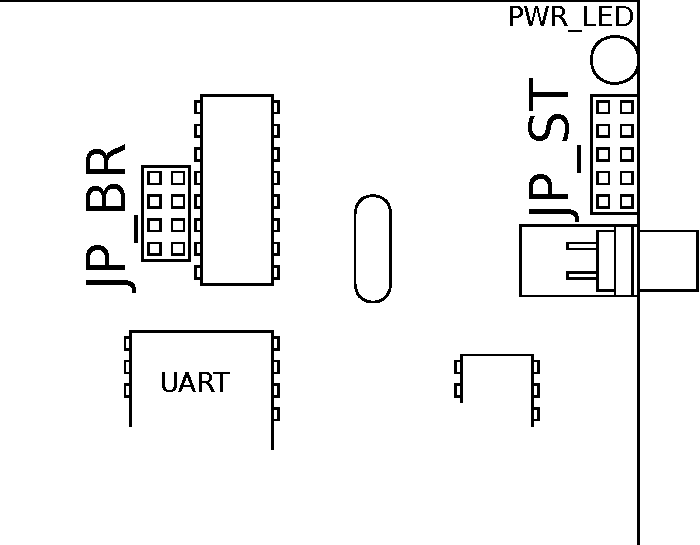
\includegraphics[width=10cm]{uart_jumpers.pdf}
 \end{center}
 \caption{Jumper locations for UART settings}
 \label{fig:jumperlocations}
\end{figure}
There are two sets of jumper headers that affect the UART, these are JP\_BR and JP\_ST shown in Figure \ref{fig:jumperlocations}.  These headers are on the lower board near the serial port and the UART chip itself.  The settings are detailed below.
\subsubsection{JP\_BR: Baud Rate}
JP\_BR connects the clock source to the UART.  This allows the baud-rate of the communications to be selected from 4 possible speeds.  Table \ref{tab:jpbr} shows the possible speed settings.

\textbf{IMPORTANT NOTE:} It is essential to fit only one jumper in one of the four positions shown on JP\_BR, connecting more will short out the clock chip's outputs!

\begin{table}[h]
 \begin{tabular}{| l | l |}
  \hline
  
\includegraphics[width=2cm]{jpbr1.pdf}&4800\\
  \hline
  
\includegraphics[width=2cm]{jpbr2.pdf}&9600\\
  \hline
  
\includegraphics[width=2cm]{jpbr3.pdf}&2400\\
  \hline
  
\includegraphics[width=2cm]{jpbr4.pdf}&19200\\
  \hline
 \end{tabular}
 \caption{Baud rate jumper positions}
 \label{tab:jpbr}
\end{table}

\subsubsection{JP\_ST: UART settings}
The five jumpers on JP\_ST can be fitted in a variety of combinations to affect the character length, parity settings and stop bits.  Table \ref{tab:jpst} describes what the individual settings do.  Some of the jumpers work in combination.  In the table, positions which are shaded have no affect on the current setting, positions which are not shaded must be either fitted or not fitted as shown.

\begin{table}[h]
 \begin{tabular}{| l | p{8cm} |}
  \hline
  
\includegraphics[height=2cm]{jpst_np.pdf}&No parity.\\
  \hline
  
\includegraphics[height=2cm]{jpst_ep.pdf}&Even parity.\\
  \hline
  
\includegraphics[height=2cm]{jpst_op.pdf}&Odd parity.\\
  \hline
  \hline
  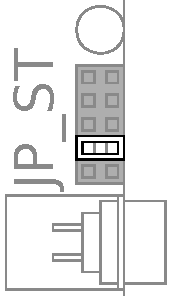
\includegraphics[height=2cm]{jpst_1sb.pdf}&One stop bit.\\
  \hline
  
\includegraphics[height=2cm]{jpst_2sb.pdf}&1.5 stop bits for character length of 5, 2 stop bits for all other lengths.\\
  \hline
  \hline
  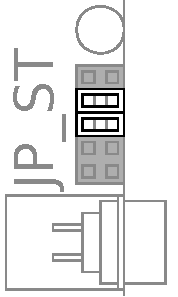
\includegraphics[height=2cm]{jpst_5b.pdf}&5 bit character.\\
  \hline
  
\includegraphics[height=2cm]{jpst_6b.pdf}&6 bit character.\\
  \hline
  
\includegraphics[height=2cm]{jpst_7b.pdf}&7 bit character.\\
  \hline
  
\includegraphics[height=2cm]{jpst_8b.pdf}&8 bit character.\\
  \hline
 \end{tabular}
 \caption{UART configuration jumpers.}
 \label{tab:jpst}
\end{table}

\chapter{GPU Commands}
\section{GPU Ports}
The GPU has two ports on the IO bus, both are read/writeable.  These are
referred to as GPU\_COMMAND (0x04) and GPU\_DATA (0x05).  The function of the
GPU\_DATA port has a constantly defined function, the command port accepts a set
of pre-defined commands which affect the way that the GPU functions.

\subsection{GPU\_DATA}
The GPU\_DATA port accepts data bytes and writes them to the active buffer.  By
default this is a display buffer so the bytes should be ASCII character codes 
corresponding to characters to be displayed on the screen.  Other data modes 
handle data in different ways, see the descriptions of these modes associated
with their commands.  By default all writes are done in ``overwrite'' mode, i.e.
whatever data is currently at the cursor is replaced with the byte written, it
is not shifted on, the cursor is automatically incremented.

Reading the data port will return a character from the cursor within the active
buffer.

\subsection{GPU\_COMMAND}
The GPU\_COMMAND port takes byte-wide commands which are used to set variables
within the GPU, and switch modes, e.g. select colour, row, or active screen.
GPU commands are basically 4 bit long in the upper nibble of the byte.  The
lower four bits are used to convey bits of data to the GPU or flags depending on
what the command is.  A summary of commands is in Table \ref{tab:gpucommands}
and details follow.

\begin{table}
 \begin{tabular}{llp{7cm}}
  \textbf{Bits}&\textbf{Name}&\textbf{Description}\\
  0000\_0000&GPU\_RESET&Issues a reset, clears all screens sets colour to 0 on all
  screens and sets both TV and VGA to virtaul screen 1.\\
  0001\_0000&GPU\_CLS&Clear screen, clears the current screen and sets cursor to
  (0,0).  The colour is not affected.\\
  0010\_bccc&GPU\_COLOUR&If b is set this sets the colour on the current screen
  to colour ccc (colours are 0-7).\\
  0011\_b000 n&GPU\_COLUMN&If b is set this sets the column on the current screen
  to the next byte sent to the command port (n).\\
  0100\_b000 n&GPU\_ROW&If b is set this sets the row on the current screen to the
  value of the next byte sent to the command port (n).\\
  0101\_0yyy&GPU\_SET\_VGA&Set the VGA to view virtual screen yyy.  (Only screens
  0 to 3 are implemented so far.)\\
  0101\_1yyy&GPU\_SET\_TV&Set the TV to view virtual screen yyy.  (Only screens 0
  to 3 are implented so far.)\\
  0110\_yyyy&GPU\_SELECT\_SCREEN&Set the active screen to virtual screen number
  yyyy.  (Currently only screens 0 to 3 are implemented, screens above 7 are
  intended to be non-display buffers)\\
  0111\_bmmm&GPU\_MODE&Set the GPU mode (VGA output only, see Section 
  \ref{sec:gpumodes} for details).  If b is set then the mode is set to mmm, if 
  b is 0 then the mode is available for read from the command port.\\
  1000\_0000&GPU\_AVAILABLE\_MODES&Get the highest mode currently detected to be
  supported by the attached screen.\\
 \end{tabular}
 \caption{GPU Command summary}
 \label{tab:gpucommands}
\end{table}

\section{GPU Modes}
\label{sec:gpumodes}
The GPU can display output in different resolutions depending on the hardware
attached.  These are called modes.  Two commands affect the mode setting and get
info about the current and available modes.  The GPU\_MODE command provides the
ability to set or get the current mode on the VGA output.  The
GPU\_AVAILABLE\_MODES command returns the highest mode that the current monitor
has been detected to support.  To allow for incorrect monitor detection, the GPU
does not prevent selection of a mode that has not been detected as supported, it
is advised that the software provides a prompt if deliberately exceeding the
recommended highest setting and reverts if no input was received in a time
period.

\vspace{12pt}
\noindent
\begin{tabular}{llp{7cm}}
 \textbf{Mode}&\textbf{Resolution (Chars)}&\textbf{Description}\\
 0&512x480 (32x15)&Low res-mode, matches TV output.  16x16 or 16x32 pixel tiles,
 4 colours per tile.  Suitable for tile based graphics or TV based text
 display.\\
 1&640x480 (80x40)&Text mode.  Supports two colours per character row, with
 8x12 characters.  Suitable for console displays etc.\\
 2&1024x768 (128x64)&Hi-res text mode.  Supports two colours per character row,
 with 8x12 pixel characters.  Suitable for console displays and text based GUIs
 on modern TFT displays of 15'' or bigger.\\
\end{tabular}

The GPU can detect a monitor attached to the VGA port that supports 640x480 or
1024x768.  If either of these modes is detected on startup the GPU selects the
640x480 text mode and puts the TV-output into sleep mode.  Querying the
supported modes will provide a value of 2 if a 1024x768 capable display has been
detected or a 1 if the display is capable of only 640x480.  If no display is
found on the VGA port at startup then this means either there is none or it does
not support plug-and-play detection.  In this case the GPU reverts to the
512x480 tile based mode, the TV display is then driven with the same output so
either display can be used as the primary output.

Once booted it is possible to switch to any other mode by sending a set mode
command.  This can be used for instance to switch to ``graphical mode'' where
the fast 16x16 tile mode can be used to generate low colour images.

When a mode switch command is issued the GPU\_READY bit in the status register is
set.  This bit is cleared again once the GPU has finished switching modes.
Commands and data sent in this time may not be handled correctly so it is
recommended not to send any.

\chapter{Keyboard Controller}
% keyboard driver documentation

\section{Keyboard Controller Commands}
You can set various keyboard parameters by writing to the KEY\_DATA port.  The
basic format for these commands is an upper nibble specifiying the command and
some parameters in the lower nibble (allowing a total of 16 commands).

\begin{tabular}{llp{6cm}l}
 \textbf{Command}&\textbf{Name}&\textbf{Description}&\textbf{Default}\\
 1100xxxx&KB\_SET\_TM&Sets the translation mode to xxxx, this is an internal 
                      setting that defines what bytes are sent to the Z80 on
                      keypress. See Table \ref{tab:translators} for details on 
                      implemented translations.& 1 (ASCII)\\
 1101000x&KB\_SET\_REL&If x is 1, all subsequent ``normal keys'' will send
                       release codes (0xF0 followed by keycode) on release.&0\\
 1110000x&KB\_SET\_CMD\_REL&If x is 1, all subsequent control keys will send
                            release codes (0xF0 followed by keycode on release.
 &1\\
 11110xxx&KB\_SET\_LEDS&This command sets the LEDs (and internal state flags)
                        to xxx.  The MSb is CAPS Lock, the middle is NUM Lock
                        and the LSb is SCROLL Lock.&010\\
\end{tabular}

\section{Translation Modes}
In the firmware implementation a relatively abstract lookup mechanism called
translate\_key is included.  This allows arbitrary byte patterns to be sent on
any keypress.  The specifications of these translators is in the following
sections, they can be selected with the KB\_SET\_TM command.  Table
\ref{tab:translators} has a summary list of available translator functions.

\begin{table}
 \begin{tabular}{rlp{7cm}}
  \textbf{Number}&\textbf{Name}&\textbf{Description}\\
  0&None&No translation is done, LEDs are kept up to date and Pause/Break is
         filtered to send only one byte.  F7 will also send 0xF7 instead of 0x83
         other than that all key-press related codes will be sent as Set 2
         scancodes.\\
  1&ASCII&Keycodes that map directly will be sent as ASCII codes these are
          ``normal keys'' which won't send release info by default.  Command
          keys (e.g. shift, ctrl, cursor keys etc.) will send custom ndcodes
          which guarantee 1 byte identification.  They will send release info
          by default.\\
 \end{tabular}
 \caption{Translation Modes}
 \label{tab:translators}
\end{table}

\section{ASCII Mode Codes}
In ASCII Mode, printable characters will be sent, CAPS, SHIFT and NUM are taken
into account before the byte is sent.  In addition keys with direct mapping to
ASCII codes will be sent as ASCII (Del = 127, Backspace = 8, Tab = 9, Return and
Enter = 10).  The only exceptions to this are two (UK) keyboard keys that don't
map to standard ASCII codes, £ and ¬.  The £ symbol is mapped to 0xA3, which 
matches the GPU's internal font mapping, the ¬ symbol has no representation in
the GPU and is replaced with a degrees symbol 0xB0.  Neither of these codes are
used in ndcodes to avoid confusion.

Other keys are sent as ndcodes which is a simple mapping which makes sure bit 7
is set for all control keys and assigns a single unique byte to each key.  These
are shown in the table below.

\subsection{Control Keys}
\begin{tabular}{llp{7cm}}
 \textbf{Mnemonic}&\textbf{Hex}&\textbf{Description}\\
 CC\_ESC&0x80&Escape\\
 CC\_F1&0x81&F1\\
 CC\_F2&0x82&F2\\
 CC\_F3&0x83&F3\\
 CC\_F4&0x84&F4\\
 CC\_F5&0x85&F5\\
 CC\_F6&0x86&F6\\
 CC\_F7&0x87&F7\\
 CC\_F8&0x88&F8\\
 CC\_F9&0x89&F9\\
 CC\_F10&0x8A&F10\\
 CC\_F11&0x8B&F11\\
 CC\_F12&0x8C&F12\\
 CC\_PRINT&0x8D&Print Screen\\
 CC\_SCROLL&0x8E&Scroll Lock\\
 CC\_PAUSE&0x8F&Pause/Break\\
 CC\_NUM&0x90&Num Lock\\
 CC\_CAPS&0x91&Caps Lock\\
 CC\_LSHIFT&0x92&Left Shift\\
 CC\_RSHIFT&0x93&Right Shift\\
 CC\_CTRL&0x94&Left Control\\
 CC\_CTRLR&0x95&Right Control\\
 CC\_ALT&0x96&Left Alt\\
 CC\_ALTR&0x97&Right Alt\\
 CC\_GUIL&0x98&Left GUI (Windows key)\\
 CC\_GUIR&0x99&Right GUI (Windows key)\\
 CC\_APPS&0x9A&Apps (Looks like a menu on most keyboards next to Windows Key\\
 CC\_INS&0x9B&Insert\\
 CC\_HOME&0x9C&Home\\
 CC\_END&0x9D&End\\
 CC\_PGUP&0x9E&Page Up\\
 CC\_PGDN&0x9F&Page Down\\
 CC\_PSF&0xA0&Fake scan code, trapped internally.\\
 CC\_PSR&0xA1&Print Screen\\
 \multicolumn{3}{c}{0xA3 is £ symbol in our character set, don't use it here}\\
 CC\_LEFT&0xA4&Left cursor key\\
 CC\_RIGHT&0xA5&Right cursor key\\
 CC\_UP&0xA6&Up cursor key\\
 CC\_DOWN&0xA7&Down cursor key\\
\end{tabular}

\subsection{Media Keys}
\begin{tabular}{llp{7cm}}
 CC\_MNXT&0xA7&Media next\\
 CC\_MPRV&0xA8&Media previous\\
 CC\_MPP&0xA9&Media play/pause\\
 CC\_MSTP&0xAA&Media stop\\
 CC\_MMT&0xAB&Media mute\\
 CC\_MVU&0xAC&Media volume up\\
 CC\_MVD&0xAD&Media volume down\\
 CC\_MSL&0xAE&Media select\\
 CC\_MEM&0xAF&Media email\\
 \multicolumn{3}{c}{0xB0 is the degrees symbol in our character set}\\
 CC\_MCLC&0xB1&Media calculator\\
 CC\_MCMP&0xB2&Media my computer\\
 CC\_MSRCH&0xB3&Web search\\
 CC\_MHOME&0xB4&Web home\\
 CC\_MBCK&0xB5&Web back\\
 CC\_MFWD&0xB6&Web forward\\
 CC\_MWSP&0xB7&Web stop\\
 CC\_MRFSH&0xB8&Web refresh\\
 CC\_MFV&0xB9&Web favourites\\
\end{tabular}

\subsection{ACPI Control Keys}
\begin{tabular}{llp{7cm}}
 CC\_PWR&0xBA&Power\\
 CC\_SLP&0xBB&Sleep\\
 CC\_WK&0xBC&Wake\\
 
\end{tabular}


\chapter{PIC Pin Allocations}
Figure \ref{fig:picpinout} shows the functions of all the pins on the PIC.  The crystal, power, programming and reset wiring have been left out for clarity.  The high address latch is fed from the low address bus, with a straight through mapping (i.e. A0 latches into A8, A2 latches into A9 ... A7 latches into A15).

\begin{figure}[h]
 \begin{center}
  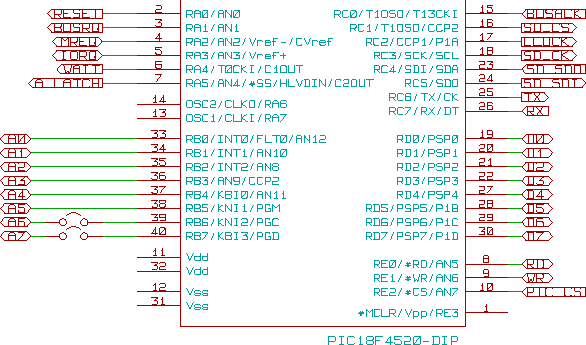
\includegraphics[width=10cm]{pic_pinout.pdf}
 \end{center}
 \caption{Pin allocations on the PIC.}
 \label{fig:picpinout}
\end{figure}

\chapter{PIC Source Structure}
The source code for the CPU supervisor PIC is split into a number of files (as of 17 Oct 2009) to aid development by compartmentalising code to make it easier to find, and also to make it easier to write ``clean'' code with minimal cross-references between blocks of different functions.  The main source files are laid out below, as well as these assembly files there are 2 other files (as well as an include file and linker script from GPUtils); the Makefile which automates building and programming the PIC and the portpins.inc file which declares the pinout of the PIC in handy names for bit-set/bit-test type operations.

\section{Files}
\subsection{Main (main.asm)}
The Main assembler file contains the glue functions that sticks all the other source files together.  This sets up the interrupt address dispatching, the initialising code and the main loop.

\subsubsection{External Functions}
There are no externally callable functions in Main.

\subsubsection{Internal Functions}

\subsubsection{Global Variables}
\begin{tabular}{lp{8cm}}
 \textbf{Name}&\textbf{Description}\\
 \texttt{MAIN\_TEMP}&A general purpose temporary register for use in the main thread (not interrupts).  Use this only for short term storage where the value will be immediately consumed by a called function or it might be overwritten.\\
\end{tabular}


\subsection{Serial (serial.asm)}
The serial assembler file contains all the code relating to the RS232 debug port on the PIC.  This code is used to allow a PC to control the Z80 CPU by giving access to DMA, with IO and Memory read and write commands.  This source file contains all the functions from the basic send and receive up to the specific command handler functions.  For details of the communications protocol and command codes see Chapter \ref{chap:comms}.

\subsubsection{External Functions}
\begin{tabular}{lp{8cm}}
 \textbf{Name}&\textbf{Description}\\
 \texttt{serial\_init}&Initialisation routine for all hardware and software set up for the serial comms routines.  Called by \texttt{init} in the main file when the PIC is started up.\\
 \texttt{serial\_rx\_int}&The interrupt handling routine.  Called from the main interrupt service in main.asm when a serial receive interrupt event occurs.\\
 \texttt{serial\_command\_dispatch}&Command dispatcher, called from the main loop.  This checks to see if there are any commands waiting to be run and directs execution accordingly.\\
\end{tabular}


\subsubsection{Internal Functions}

\subsubsection{Global Variables}

\subsection{Z80 Bus (host\_bus.asm)}
The Z80 Bus assembler file contains all the functions for accessing the host CPU bus, e.g. writing to an IO port, or putting the Z80 into DMA slave mode.  See the sd\_card.asm section for the Slave device functions.

\subsubsection{External Functions}
\begin{tabular}{lp{8cm}}
 \textbf{Name}&\textbf{Description}\\
 \texttt{get\_reset}&Call this function to put the Z80 into reset and set the PIC as the bus master.\\
 \texttt{get\_dma}&Call this function to put the Z80 into DMA mode and set the PIC as the bus master.\\
 \texttt{get\_slave}&Set the PIC to be a normal IO device on the bus.  This releases control of the bus and releases the RESET and BUSRQ lines, it also enables interrupts on the PSP so that read/write from the PIC is handled by interrupt.\\
 \texttt{ensure\_master}&Call this to make sure that the Z80 is master, if it is this returns immediately, if not it puts the Z80 into DMA slave mode.  This is designed to allow random access to peek at memory or peripherals without setting up a master session manually each time, but allows for a master session to be set up by first calling \texttt{get\_reset} or \texttt{get\_dma}.\\
 \texttt{revert\_master}&Call this after a call to \texttt{ensure\_master} to return the bus to the previous state (e.g. PIC as slave etc.)\\
 \texttt{io\_read}&Read a single IO address, the address is taken from \texttt{HI\_ADDR} and \texttt{LO\_ADDR}, data is returned in \texttt{DREG}.  No mode checking is performed when this is called so it is the calling routine's responsibility to check that the PIC is allowed to drive the bus.\\
 \texttt{io\_write}&As with \texttt{io\_read} except that the content of \texttt{DREG} are written to the address provided.\\
 \texttt{mem\_read}&Identical to \texttt{io\_read} except that it drives the memory bus instead.\\
 \texttt{mem\_write}&Identical to \texttt{io\_write} except that it drives the memory bus instead.\\
\end{tabular}

\subsubsection{Internal Functions}

\subsubsection{Global Variables}
\begin{tabular}{lp{8cm}}
 \textbf{Name}&\textbf{Description}\\
 \texttt{HI\_ADDR}&High byte of address for bus operations.\\
 \texttt{LO\_ADDR}&Low byte of address for bus operations.\\
 \texttt{DREG}&Data buffer for bus operations.\\
\end{tabular}


\subsection{SD Card Functions (sd\_card.asm)}
When the PIC is in peripheral mode it sits on the bus acting as a pass-through device for accessing an SD card in MMC (SPI) mode.  This allows the Z80 to do simple byte operations to it even though the SD card interface is serial.  The PIC does not do any of the file system handling or higher functions though.  The main interface to this code is interrupt driven from the PSP peripheral on the PIC.

\subsubsection{External Functions}

\subsubsection{Internal Functions}

\subsubsection{Global Variables}

\subsection{Z80 Boot (boot.asm)}
The Z80 boot file contains a few high level functions that are used to allow the system's boot ROM to be stored in the PIC's flash memory.  This code is called at start-up to copy the boot ROM into system RAM.  There is also support for sending the boot code to the host PC and for downloading a new boot code from the host PC within this source file.

\subsubsection{External Functions}
\begin{tabular}{lp{8cm}}
 \textbf{Name}&\texttt{Description}\\
 \texttt{boot\_init}&Setup all the external functions for driving the Z80.  This is mainly to do with the software-generated clock signal that is made by one of the PIC's PWM peripherals.\\
 \texttt{boot\_load}&Copies the ROM image from the top 8K of the PIC's Flash into the bottom 8K of the system memory map.\\
 \texttt{boot\_update}&Copies a 128 byte block from the RX buffer to the internal Flash.\\
\end{tabular}


\subsubsection{Internal Functions}

\subsubsection{Global Variables}

\subsection{Boot ROM (rom.asm)}
This file has no functions, it contains a chunk of Z80 machine code that is used to boot the main CPU after it is copied to system RAM on boot.  This file provides a convenient way to include the code in to the final hex file for the PIC.

\subsubsection{External Functions}
There are no external functions in this file.

\subsubsection{Internal Functions}
There are no internal functions in this file.

\subsubsection{Global Variables}

\chapter{Variables and Constants}


\chapter{Debug Comms Protocol}
\label{chap:comms}
\section{Buffer Locations}
RX Buffer: 0x0100-0x01FF, Used through INDF0\\
TX Buffer: 0x0200-0x02FF, Used through INDF1

\section{Packet Specifications}
\subsection{Host to Device Packet Definition}
\begin{tabular}{l|c|p{6cm}}
 \textbf{Name}&\textbf{Length (Bytes)}&\textbf{Description}\\
\hline
 Command&1&A byte in the range 0x00-0x1F (0-31) See the instruction table below for details.\\
\hline
 Data Length&1&Length (in bytes) of the data payload of the packet.  Maximum value is 253 so that the whole packet fits into the buffer.\\
\hline
 Data&\textit{data length}&Any byte string specified by the length.  Can be zero length.\\
\hline
 Checksum&1&An XOR checksum of all the bytes in the packet from the Command to the last byte of the data.\\
\end{tabular}

\subsection{Device to Host Packet Definition}
\begin{tabular}{l|c|p{6cm}}
 \textbf{Name}&\textbf{Length (Bytes)}&\textbf{Description}\\
\hline
 Response&1&A Response code.  Normally based on the command that this is responding to.  See the response code details below.\\
\hline
 Data Length&1&Length (in bytes) of the data payload of the response.  Any value from 0-253 is valid, but depends on what the expected response requires.\\
\hline
 Data&\textit{data length}&The byte string being returned.  This is not included for a simple acknowledge message.\\
\hline
 Checksum&1&An XOR checksum of the response packet.\\
\end{tabular}

\section{Response Codes}
As was stated in the above table the response code is normally just the command code that the response belongs to.  However there are several exceptions to this.  The simplest is the error response.  If an error occurs (e.g. the wrong number of parameters are provided for a command or the command does not do anything) an error packet is sent back to the host.  The response code in this case is the command code with bit 6 set (i.e. a bitwise and with 0x40).  Hence if command 0x0A encounters an error, the response code would be 0x4A.

In cases where the error could cause corruption of the command code or the code was invalid the PIC will never send an un-defined code, instead it responds with a special code with bit 7 set (0x80-0xFF).  For example if the checksum fails, the error may be in the command, so it is not sent back to the PC, instead 0x80 is used.  These `special' responses are in the special column of the error codes table below.

\section{Command Codes}
There are 32 command codes numbered sequentially from 0 to 31.  If a command is listed as `Unused' then it will respond with an ``Unused Command'' error packet.  The parameters are what is transmitted in the payload of the packet, in the order listed.  Addresses are transmitted Big Endian (i.e. high byte first).  The Mnemonic field is a simple text string representing the value for clarity of code, this is what is included in the seriallib Python library for example.

\subsection{Summary}
\begin{tabular}{|r|l|p{3cm}|p{4.5cm}|}
\hline
 \textbf{Code}&\textbf{Mnemonic}&\textbf{Description}&\textbf{Parameters}\\
\hline
 0&None&Reserved&\\
\hline
 1&None&Unused&\\
\hline
 2&RDMEM&Read Mem&Address High (1 Byte)\\
&&&Address Low (1 Byte)\\
\hline
 3&WRMEM&Write Mem&Address High (1 Byte)\\
&&&Address Low (1 Byte)\\
&&&Data (1 Byte)\\
\hline
 4&RDMEMBLK&Block Mem Read&Start Address High (1 Byte)\\
&&&Start Address Low (1 Byte)\\
&&&Length (1 Byte)\\
\hline
 5&WRMEMBLK&Block Mem Write&Start Address High (1 Byte)\\
&&&Start Address Low (1 Byte)\\
&&&Data Block (\textit{Length}-2 Bytes)\\
\hline
 6&RDIO&Read IO&Address High (1 Byte)\\
&&&Address Low (1 Byte)\\
\hline
 7&WRIO&Write IO&Address High (1 Byte)\\
&&&Address Low (1 Byte)\\
&&&Data Byte (1 Byte)\\
\hline
 8&UPDBIOS&Update BIOS&Start Address High (1 Byte)\\
&&&Start Address Low (1 Byte)\\
&&&Data (128 Bytes)\\ 
\hline
 9&DOCMD&Do Command&Command code (1 Byte)\\
\hline
 10&None&Unused&\\
\hline
 11&None&Unused&\\
\hline
 12&None&Unused&\\
\hline
 13&None&Unused&\\
\hline
 14&None&Unused&\\
\hline
 15&None&Unused&\\
\hline
 16&None&Unused&\\
\hline
 17&None&Unused&\\
\hline
 18&None&Unused&\\
\hline
 19&None&Unused&\\
\hline
 20&None&Unused&\\
\hline
 21&None&Unused&\\
\hline
 22&None&Unused&\\
\hline
 23&None&Unused&\\
\hline
 24&None&Unused&\\
\hline
 25&None&Unused&\\
\hline
 26&None&Unused&\\
\hline
 27&None&Unused&\\
\hline
 28&None&Unused&\\
\hline
 29&None&Unused&\\
\hline
 30&None&Unused&\\
\hline
 31&None&Unused&\\
\hline
\end{tabular}

\subsection{Mem Block Write}
The memory block write command writes a block of data to the main memory at the location specified in the command.  The first data byte specifies the upper address byte for the start point, and the second is the lower address byte.  The rest of the data bytes (the packet length field - 2) are then written to memory starting at this address, so a total of 251 bytes may be written in one go.  The address is incremented after each write so the byte order for the frame is little endian, this is opposite to the address byte order.

\subsection{BIOS Update}
The Z80 BIOS is stored in the PIC's internal Flash memory and copied to the system at boot.  The BIOS can be updated through the PIC's debug serial port without re-programming the whole PIC firmware.  This is done in chunks of 128 bytes.  There is no requirement to update all 8K of the BIOS image at the same time, nor do you have to do it in any particular order.  Each 128 byte block must be aligned at a 128 byte offset (i.e. bits <6:0> of the address need to be 0).  The address is the address within the BIOS itself, the PIC will automatically redirect writes to the appropriate part of Flash, so an address in the range 0x0000-0x1F80 is valid. On successful write of the block an ACK will be sent, if the parameters given are not acceptable various error messages may be produced (see below).  If the write fails verification, a 0x0007 error message is sent.  In this case simply try this block again as the BIOS storage space doesn't affect the PICs operation in anyway the debug kernel cannot be damaged by a failed BIOS update.  Operation of the Z80 if a reset is performed is likely to go wrong.

\subsection{Do Command}
The Do Command instruction is a special instruction which is used for executing simple no-data instructions, e.g. reset.  The packet contains a single data byte which is the name of the instruction to execute (there are up to 256 instructions 0x00-0xFF).  The response is simply the same packet, or an error code, none of the ``Do'' subset of commands can reply with any data.

\begin{tabular}{|r|l|p{7cm}|}
 \hline
 \textbf{Do Code}&\textbf{Mnemonic}&\textbf{Description}\\
 \hline
 0&None&Reserved\\
 \hline
 1&DOGETRST&Pull Z80 Reset line low until further notice.\\
 \hline
 2&DOGETDMA&Put the Z80 into DMA slave mode until further notice.\\
 \hline
 3&DOGETSLA&Release the Z80 into normal run mode, make the PIC a slave device.\\
 \hline
 4&DORST&Issue a software Reset to the PIC.  Resets the whole system, wiping RAM and re-bootin the Z80 from the stored ROM image.\\
 \hline
 Other&None&Not defined, will return Error 9.\\
 \hline
\end{tabular}

\section{Error Messages}
The minimum length for an error packet is 2 Bytes.  The first two bytes of the error packet are always an error code to indicate what the problem is.  In some cases where more information is available this is included after the error number, for example if the wrong number of bytes were sent with the command the number of bytes expected is specified in the response packet.  The error codes are specified below, in the error packet the high byte of the error code comes first (directly after the length field) followed by the low byte.

\begin{tabular}{|r|c|p{3.7cm}|p{3.7cm}|}
\hline
\textbf{Code}&\textbf{Special}&\textbf{Description}&\textbf{Additional Data}\\
\hline
0&&No error&None\\
\hline
1&0x80&Checksum Error&The checksum calculated by the PIC (1 Byte)\\
\hline
2&0x81&Bad Command (greater than 31)&The code the PIC received.\\
\hline
3&&Unused Command&\\
\hline
4&&Wrong number of parameters&The correct number for this command.\\
\hline
5&&The requested data is too big for one packet&\\
\hline
6&&The start address for BIOS update was not within a valid range (max 0x1FFF)&\\
\hline
7&&The offset for the BIOS was not aligned to the 128 byte packet size.&\\
\hline
8&&There was a verification error for this BIOS update.&\\
\hline
9&&Unknown do command.&The unknown command.\\
\hline
\end{tabular}

\section{seriallib.py}
\texttt{seriallib.py} is a Python library which automates a lot of the basic processing functions of the protocol.  Include it in a project by placing a copy in your Python path, or in the project folder then adding the line \texttt{include seriallib}.  Within the library are constants to save remembering the numerical values of commands e.g. typing \texttt{seriallib.DOCMD} will be treated as an integer of value 9 (the command code for a Do Command packet).  The rest of the fucntionality is wrapped in classes.

\subsection{Packet}
The Packet class is a representation of the packet type which automates length calculation and checksum generation whilst maintaining the flexibility of a string.  Specific bytes can be read from it as from a string using subscripting e.g. the length of the packet may be retreived as a character type from a packet \texttt{pkt} by subscripting byte 1; \texttt{pkt[1]}.  Other string like functions that work with the packet are \texttt{len()} which returns the total byte length of the packet (including command, length and checksum bytes, so the number is equal to the length field + 3).  Calling \texttt{str()} on the packet will return the byte string in a binary form i.e. there may be non-printable characters within it.  This is the default representation used if you \texttt{print} the packet.  To gain a more useful insight into the contents of the packet, calling \texttt{repr()} on it will return the whole packet as 2 digit, zero padded hexadecimal values separated by spaces, so for example a Do Get Reset command would appear as \texttt{09 01 01 09}.

\subsubsection{Assigning Packet Values}
There are two ways to assemble a packet using the \texttt{Packet} class.  The best way for assembling a packet to transmit is by calling the \texttt{set\_command} and \texttt{set\_data} methods.  \texttt{set\_command} expects an integer between 0 and 31 which it will validate and convert to a byte for transmission, this is ideal for use with the constants declared to make code more readable.  The \texttt{set\_data} command expects a string which does not need to be printable characters, this forms the data payload of the packet un-altered.  If you pass a small integer (less than 256) to \texttt{set\_data} it will convert it to a single character.  This is useful for using the Do Command integer constants, if a larger number is given it will produce an error.  Note that \texttt{set\_data} does not append to existing data so you cannot build a packet a bit at a time using this method.  You do not need to set the checksum or length values as these are calculated when needed.

The other method of generating a \texttt{Packet} is using the \texttt{set\_string} method.  This takes one argument which is a byte string that is interpreted as a packet.  When you assign data this way the checksum and length fields are validated to ensure this was a valid packet, then the bytes are assigned to the internal storage.  You can then alter the command or data with the \texttt{set\_command} or \texttt{set\_data} methods, or print the packet etc.  Much more useful in the case of a received packet is the ability to get a readable error message from it.  The \texttt{Packet} class knows all the error codes and what data is returned with that type of error and will wrap this information up in a hopefully descriptive message.  This error description can be aquired with the \texttt{get\_error} method.  This returns a tuple, the first element is an integer giving the error code, the second element is a descriptive string.  The error code matches the codes presented here, where 0 is no error and higher numbers correspond to specific communications or system events.  A useful test for an error is to perform an if on element 0 of the response
\begin{verbatim}
 if pkt.get_error()[0] > 0:
    print "There was an error"
    print "  Code %d: %s" % pkt.get_error()
\end{verbatim}

\chapter{Z80 BIOS Routines}
The following routines are built into the Z80 bios.  If they are documented here
then they should be safe to call from external code.  Where this is not so, the
restrictions are noted in the description.  Functions will not alter registers
(other than A and F) unless these registers are specified as inputs or outputs.

The sources is split into a number of files which are roughly split based on the
hardware they interface to (e.g. UART, RTC etc.) or a specific duty within the
software (e.g. maths).  The filename and linenumber of the jumplabel are stated
at the start of each function description.

\section{Alphabetical List of Functions}
\begin{tabular}{rllp{7cm}}
 \textbf{Source}&\textbf{Function}&\textbf{Address}&\textbf{Description}\\
 bios.z8a:296&bios\_disable\_int&\$8036&disable interrupts flagged in byte in A\\
 bios.z8a:279&bios\_enable\_int&\$8026&enable the interrupt indicated by register A\\
 bios.z8a:248&bios\_error\_exit&\$8019&called on a fatal error after GPU is ready\\
 bios.z8a:334&bios\_load\_var&\$8054&loads a byte from non-volatile BIOS memory\\
 bios.z8a:387&bios\_reset&\$808d&ask the PIC to do a full system reset\\
 bios.z8a:315&bios\_save\_var&\$8045&saves a byte of data to non-volatile bios memory\\
 bios.z8a:264&bios\_set\_interrupts&\$801e&set PIE and the local copy of interrupt flags\\
 fat.z8a:30&fat\_init&\$8974&read a FAT boot sector and setup the FAT driver\\
 fat.z8a:476&fat\_next\_block&\$8bf3&fetch the next block in the current file/folder.\\
 fat.z8a:531&fat\_next\_cluster&\$8c36&fetch the next cluster of the active file\\
 fat.z8a:308&fat\_select\_cluster&\$8b0a&(re)initialise the FAT firmware pointing at a specific cluster.\\
 gpu.z8a:47&gpu\_cls&\$8099&Clear the active screen\\
 gpu.z8a:182&gpu\_dec&\$80f3&Print a decimal value to the screen, maximum of 32bit input\\
 gpu.z8a:79&gpu\_get\_colour&\$80a7&Return the active colour from the GPU\\
 gpu.z8a:212&gpu\_hex&\$8108&Print a hex representation of a number\\
 gpu.z8a:33&gpu\_init&\$8094&Reset the GPU to its power-on state\\
 gpu.z8a:63&gpu\_set\_colour&\$809e&Select the colour on the active screen\\
 gpu.z8a:161&gpu\_str&\$80e9&Print a null terminated string\\
 maths.z8a:255&maths\_add32&\$843b&Add maths\_op\_b to maths\_op\_a and store in maths\_op\_a\\
 maths.z8a:192&maths\_asl32&\$841d&shift maths\_op\_a one bit left and put a zero in the lsb\\
 maths.z8a:215&maths\_asln32&\$8425&shift maths\_op\_a n bits left and zero the new lsbs\\
 maths.z8a:122&maths\_asr32&\$83fb&32 bit arithmetic shift right\\
 maths.z8a:148&maths\_asrn32&\$8403&32 bit arithmetic shift right by n bits\\
 maths.z8a:27&maths\_bcd\_to\_bin&\$83b7&convert a single byte from BCD to binary (in a)\\
 maths.z8a:628&maths\_bin\_to\_bcd&\$8605&convert a 32\textit{24}16\\
 maths.z8a:389&maths\_div32&\$84de&calculate the div\\
 maths.z8a:48&maths\_mod&\$83c9&calculate a/b - returns b unaltered, a = a \% b, c = a//b\\
 maths.z8a:321&maths\_sub32&\$848e&do a 32 bit subtraction maths\_op\_a - maths\_op\_b\\
 maths.z8a:594&maths\_test\_z32&\$85ed&test a 32 bit value for zero\\
 maths.z8a:575&maths\_test\_z64&\$85e4&test a 64 bit value for zero\\
 uart.z8a:53&uart\_write&\$8169&Writes the contents of \textbf{A} to the UART\\
 usb.z8a:32&usb\_get\_byte&\$8d1c&read a byte from the Vinculum chip.\\
 usb.z8a:48&usb\_write\_byte&\$8d25&write a byte to the Vinculum chip\\
\end{tabular}

\subsection{bios\_disable\_int}
\textit{bios.z8a:296 - \$8036}

\noindent
\textbf{disable interrupts flagged in byte in A}

\subsubsection{No Documentation}


\subsection{bios\_enable\_int}
\textit{bios.z8a:279 - \$8026}

\noindent
\textbf{enable the interrupt indicated by register A}

\subsubsection{Description:}
 Register A contains a bit mask with a 1 in every interrupt to enable.  This is carried out and the updated value recorded in system\_interrupts.  The interrupt enable is set at the end so don't call from interrupts.

\subsection{bios\_error\_exit}
\textit{bios.z8a:248 - \$8019}

\noindent
\textbf{called on a fatal error after GPU is ready}

\subsubsection{Description:}
 This function is called by BIOS functions on errors, but only after the GPU has been started.  When called \textbf{HL} contains a pointer to a string with some information about the error, this is printed then the system is halted.

\subsection{bios\_load\_var}
\textit{bios.z8a:334 - \$8054}

\noindent
\textbf{loads a byte from non-volatile BIOS memory}

\subsubsection{Description:}
 \textbf{A} is loaded with a byte fetched from location \textbf{B} from EEPROM memory.

\subsection{bios\_reset}
\textit{bios.z8a:387 - \$808d}

\noindent
\textbf{ask the PIC to do a full system reset}

\subsubsection{Description:}
 In some cases it is useful to be able to reboot (after setting BIOS parameters for example.)  In these cases it's important that all the support circuits get reset as well to enable proper boot, issuing a command to the supervisor PIC can tell it to do a full system-reset.

\subsection{bios\_save\_var}
\textit{bios.z8a:315 - \$8045}

\noindent
\textbf{saves a byte of data to non-volatile bios memory}

\subsubsection{Description:}
 The contents of \textbf{A} are saved to the non-volatile BIOS setting storage in one of 256 locations as indicated by the contents of \textbf{B}.

\subsection{bios\_set\_interrupts}
\textit{bios.z8a:264 - \$801e}

\noindent
\textbf{set PIE and the local copy of interrupt flags}

\subsubsection{Description:}
 Because the Peripheral Interrupt Enable register is write-only, a copy of the current flag settings is stored in memory, by using this function both of the locations are kept up to date.  This is thread-safe as it blocks interrupts to ensure both locations are kept in sync so it is safe to alter the system\_interrupts value in memory from interrupts, don't call directly as it enables interrupts.  The value to set is in \textbf{A}.

\subsection{fat\_init}
\textit{fat.z8a:30 - \$8974}

\noindent
\textbf{read a FAT boot sector and setup the FAT driver}

\subsubsection{Description:}
 sd\_block should be set pointing to the start of the FAT partition before  calling this function.  It should be called before any other FAT subroutines.

\subsection{fat\_next\_block}
\textit{fat.z8a:476 - \$8bf3}

\noindent
\textbf{fetch the next block in the current file/folder.}

\subsubsection{Description:}
 Fetches the next block of the current file or folder.  On return Carry is set if the fetch failed.  If the fat\_error register is clear then it just means the end of the file was reached.

\subsection{fat\_next\_cluster}
\textit{fat.z8a:531 - \$8c36}

\noindent
\textbf{fetch the next cluster of the active file}

\subsubsection{Description:}
 This function finds the number of the next cluster in the active file/folder if there is one and calls fat\_select\_cluster to initialise that cluster. Returns directly with carry flag set and FAT\_ERROR\_NONE if there are no more clusters in the current file.  Otherwise the return is from fat\_select\_cluster.

\subsection{fat\_select\_cluster}
\textit{fat.z8a:308 - \$8b0a}

\noindent
\textbf{(re)initialise the FAT firmware pointing at a specific cluster.}

\subsubsection{Description:}
 Called after an update to fat\_cluster.  Points fat\_block to the start of the current cluster and calculates fat\_last\_block for this cluster.  Also performs error checking on the sector number, if the number is 0 it returns with carry set but no error in sd\_error, the same behaviour is used for cluster numbers higher than the highest available.  This works for FAT entry checking.  On FAT16 requesting Sector \#1 will return the first block of the root directory.  On FAT32 this will fail like requesting 0 or high numbers.

\subsection{gpu\_cls}
\textit{gpu.z8a:47 - \$8099}

\noindent
\textbf{Clear the active screen}

\subsubsection{Description:}
 This sets all pixels in the active screen to the currently selected background colour.  Reading any cursor location will return \$20 (the ASCII code for SPACE).  Register \textbf{A} is used, but no arguments or return values are associated with this function.

\subsection{gpu\_dec}
\textit{gpu.z8a:182 - \$80f3}

\noindent
\textbf{Print a decimal value to the screen, maximum of 32bit input}

\subsubsection{Description:}
 This prints a decimal representation (in ASCII characters 0-9) of a numerical value to the screen.  The number should be a normal binary number (to print BCD, call gpu\_hex).  The source is not affected, but the maths registers are used for the conversion to BCD.  HL is a pointer to the source number, \textbf{B} contains the number of ASCII characters (counted from the least significant up) to print to the screen, \textbf{A} contains a number of bytes long the number to convert is (can be 1, 2, 3 or 4).  If \textbf{A} is zero or 5 or more then 32bit is assumed.

\subsection{gpu\_get\_colour}
\textit{gpu.z8a:79 - \$80a7}

\noindent
\textbf{Return the active colour from the GPU}

\subsubsection{Description:}
 This command queries the GPU to find out what the active colour is.  This colour index is returned in \textbf{A} and must be in the range 0-7.  The actual colour this represents depends on the colour map of the GPU at the time of the request.

\subsection{gpu\_hex}
\textit{gpu.z8a:212 - \$8108}

\noindent
\textbf{Print a hex representation of a number}

\subsubsection{Description:}
 This function sends ASCII characters representing 4 bit values to the GPU to display binary values from memory.  \textbf{HL} contains a pointer to the location in memory of the bytes to represent, \textbf{A} contains a number of Hex digits to print.  When called the function starts printing nibbles from \textbf{A} above \textbf{HL} and moves down.  \textbf{HL} is not altered by this function, neither is the memory that is printed.  This function can also be used to print BCD values directly.

\subsection{gpu\_init}
\textit{gpu.z8a:33 - \$8094}

\noindent
\textbf{Reset the GPU to its power-on state}

\subsubsection{Description:}
 On start up the GPU displays a blank screen on both VGA and TV monitors.  It is in a 16x32 tile-based mode with a default colour table.  Running this command orders the GPU to return to this state.  Register \textbf{A} is used, but no arguments or return values are associated with this function.

\subsection{gpu\_set\_colour}
\textit{gpu.z8a:63 - \$809e}

\noindent
\textbf{Select the colour on the active screen}

\subsubsection{Description:}
 There are 8 colours available at any time in the GPU.  Each colour is a pair of foreground and background values selected from a possible range of 64 visible colours.  This command selects which of the eight foreground/background colour pairs from the current colour map will be used when printing characters to the active screen.\\\\ The colour to use is passed in \textbf{A} and is masked to a value 0-7.

\subsection{gpu\_str}
\textit{gpu.z8a:161 - \$80e9}

\noindent
\textbf{Print a null terminated string}

\subsubsection{Description:}
 \textbf{HL} is a pointer to the first byte of a null-terinated string.  The bytes are sent un-altered to the data port of the GPU until a null is found which causes the function to return.  \textbf{A} is altered during this function, \textbf{HL} is incremented to the end of the string, no other registers or memory locations will be written.

\subsection{maths\_add32}
\textit{maths.z8a:255 - \$843b}

\noindent
\textbf{Add maths\\\_op\\\_b to maths\\\_op\\\_a and store in maths\\\_op\\\_a}

\subsubsection{Description:}
 Performs a 32 bit addition of a value in maths\_op\_a and maths\_op\_b.  The result is stored in maths\_op\_a by default, to use maths\_op\_b or maths\_op\_c as the target call maths\_add32\_b or maths\_add32\_c.  No registers are affected by this call. maths\_op\_a + maths\_op\_b =\textgreater  maths\_op\_x (depending on call) Flags:  maths\_flags[C] is set if the addition resulted in overflow, reset otherwise  maths\_flags[Z] is set if the result of the addition was zero, reset                 otherwise

\subsection{maths\_asl32}
\textit{maths.z8a:192 - \$841d}

\noindent
\textbf{shift maths\\\_op\\\_a one bit left and put a zero in the lsb}

\subsubsection{Description:}
 The contents of maths\_op\_a are shifted one bit to the left (upwards) and a zero is placed in the least significant bit. [C] \textless - [31 \textless - 0] \textless - 0 Flags:  maths\_flags[Z] is set if the result is zero, reset otherwise  maths\_flags[C] is set if the most significant bit was 1 before the shift,                 reset otherwise The contents of internal registers are not affected by this function.

\subsection{maths\_asln32}
\textit{maths.z8a:215 - \$8425}

\noindent
\textbf{shift maths\\\_op\\\_a n bits left and zero the new lsbs}

\subsubsection{Description:}
 The contents of maths\_op\_a are shifted n bit to the left (upwards) based on the value of \textbf{A} and zeros are placed in the least significant bits. [C] \textless n- [31 \textless n- 0] \textless n- 0 Flags:  maths\_flags[Z] is set if the result is zero, reset otherwise  maths\_flags[C] is set if the last bit shifted out was 1 reset otherwise The contents of internal registers are not affected by this function, \textbf{A} is not preserved however.

\subsection{maths\_asr32}
\textit{maths.z8a:122 - \$83fb}

\noindent
\textbf{32 bit arithmetic shift right}

\subsubsection{Description:}
 The contents of maths\_op\_a are shifted one bit to the right.  The most  significant bit is left unaltered (so the sign of the number is not changed).  [31] -\textgreater  [31 -\textgreater  0] -\textgreater  [C] Flags:  maths\_flags[Z] is set if the result is zero, reset otherwise  maths\_flags[C] is set if the lsb was 1 before the operation, reset otherwise None of the CPU registers are affected by this function.

\subsection{maths\_asrn32}
\textit{maths.z8a:148 - \$8403}

\noindent
\textbf{32 bit arithmetic shift right by n bits}

\subsubsection{Description:}
 The contents of maths\_op\_a are shifted a number of bits to the right.  The number of bits to shift is specified by the contents of \textbf{A} (the value is masked to 5 bits to provide a maximum of 31 bit shift).  The most significant bit is propagated down each shift (so the sign of the number is not changed).  [31] -n\textgreater  [31 -\textgreater  0] -n\textgreater  [C] Flags:  maths\_flags[Z] is set if the result is zero, reset otherwise  maths\_flags[C] is set if the last bit shifted out of bit 0 was 1, reset  otherwise The contents of the accumulator are not preserved by this operation, other registers are unaffected.

\subsection{maths\_bcd\_to\_bin}
\textit{maths.z8a:27 - \$83b7}

\noindent
\textbf{convert a single byte from BCD to binary (in a)}

\subsubsection{No Documentation}


\subsection{maths\_bin\_to\_bcd}
\textit{maths.z8a:628 - \$8605}

\noindent
\textbf{convert a 322416}

\subsubsection{Description:}
 \textbf{HL} points to a value up to 4 bytes long to be converted, it is not altered so it is safe to point at values in ROM or that will be used later.  \textbf{HL} is the least significant byte, \textbf{A} contains the number of bytes to copy (1, 2 3 or 4) these bytes are copied to maths\_op\_b with higher bytes set to zero. The result of the conversion is stored in maths\_op\_c and may be up to 5 bytes long.

\subsection{maths\_div32}
\textit{maths.z8a:389 - \$84de}

\noindent
\textbf{calculate the div}

\subsubsection{Description:}
 The contents of maths\_op\_a are divided by the contents of maths\_op\_b.  The quotient is placed in the lower 32 bits of maths\_op\_c, the remainder is left in maths\_op\_a.  On return carry is set if it was an illegal (division by zero operation).

\subsection{maths\_mod}
\textit{maths.z8a:48 - \$83c9}

\noindent
\textbf{calculate a/b - returns b unaltered, a = a \\\% b, c = a//b}

\subsubsection{No Documentation}


\subsection{maths\_sub32}
\textit{maths.z8a:321 - \$848e}

\noindent
\textbf{do a 32 bit subtraction maths\\\_op\\\_a - maths\\\_op\\\_b}

\subsubsection{No Documentation}


\subsection{maths\_test\_z32}
\textit{maths.z8a:594 - \$85ed}

\noindent
\textbf{test a 32 bit value for zero}

\subsubsection{Description:}
 \textbf{HL} points to the least significant byte of a 32 bit value to be tested.  If the value is zero bit 1 (second least significant) of \textbf{A} is set, otherwise this bit is cleared.  This matches the \textbf{Z} bit position in the maths\_flags  register so loading \textbf{A} with the contents of flags before a call and writing it back after will update the flags register.  \textbf{HL} is left pointing 4 bytes above where it started, no other registers are affected.

\subsection{maths\_test\_z64}
\textit{maths.z8a:575 - \$85e4}

\noindent
\textbf{test a 64 bit value for zero}

\subsubsection{Description:}
 Works identically to maths\_test\_z32 but tests a total of 8 bytes starting at location \textbf{HL}.  Used in testing results of 32x32 multiply etc.

\subsection{uart\_write}
\textit{uart.z8a:53 - \$8169}

\noindent
\textbf{Writes the contents of A to the UART}

\subsubsection{Description:}
 UART write checks the status of the UART and sends once the buffer is empty. This is an indefinitely blocking call, however the UART clock can't be stopped in this system so it should always complete.

\subsection{usb\_get\_byte}
\textit{usb.z8a:32 - \$8d1c}

\noindent
\textbf{read a byte from the Vinculum chip.}

\subsubsection{Description:}
 This call fetches a single byte from the Vinculum chip.  It obeys the status flag USB\_RXF to avoid reading bytes before they are ready.  Note that it will block indefinitely for bytes to be ready so call with caution.

\subsection{usb\_write\_byte}
\textit{usb.z8a:48 - \$8d25}

\noindent
\textbf{write a byte to the Vinculum chip}

\subsubsection{Description:}
 Writes a single byte (from \textbf{A}) to the USB host chip.  The USB\_TXE flag is checked to make sure that the Vinculum is ready to accept bytes.  If there are bytes to be read these are read and discarded as the output buffer must be empty before you try writing.

\section{Alphabetical List  of Variables}
\begin{tabular}{rllp{7cm}}
 \textbf{Source}&\textbf{Function}&\textbf{Address}&\textbf{Description}\\
 gpu.z8a:285&gpu\_hex\_lut&\$8142&16 byte lookup to convert one 4 bit value to an ASCII character\\
 maths.z8a:804&maths\_flags&\$86a9&flag register holds the flags from the last maths routine\\
 maths.z8a:783&maths\_op\_a&\$8699&32 bit operator for maths routines\\
 maths.z8a:789&maths\_op\_b&\$869d&32 bit operator for maths routines\\
 maths.z8a:795&maths\_op\_c&\$86a1&64 bit result register for maths\_routines\\
 bios.z8a:111&ram\_top&\$8000&A pointer to the last byte in RAM\\
 bios.z8a:237&stack&\$9fff&The bottom of (highest address used by) the stack\\
 bios.z8a:197&system\_boot\_device&\$8017&Set by the BIOS bootloader to indicate where the boot image in use was found\\
 bios.z8a:225&system\_boot\_file&\$8018&Set by the bootloader to the path to the currently running program file loaded at boot\\
 bios.z8a:163&system\_boot\_order&\$8015&The order in which devices are searched for a boot image\\
 bios.z8a:129&system\_clock&\$8004&The speed of the Z80 clock\\
 bios.z8a:141&system\_clock\_speeds&\$8005&Lookup table to convert clock setting to Hz\\
 bios.z8a:182&system\_filesystem&\$8016&indicates the filesystem type if boot was from SD card\\
\end{tabular}

\subsection{gpu\_hex\_lut}
\textit{gpu.z8a:285 - \$8142}

\noindent
\textbf{16 byte lookup to convert one 4 bit value to an ASCII character}

\subsubsection{Description:}
 Since ASCII characters A-F do not follow 0-9 normally this is provided as a lookup to convert a 4 bit value to ASCII.\\\\ Access: Read-only

\subsection{maths\_flags}
\textit{maths.z8a:804 - \$86a9}

\noindent
\textbf{flag register holds the flags from the last maths routine}

\subsubsection{Description:}
 Bit 0: Carry, set when an add/subtract overflows. Bit 1: Zero, set when the result of the operation was zero. See commands for details about what happens to these flags.

\subsection{maths\_op\_a}
\textit{maths.z8a:783 - \$8699}

\noindent
\textbf{32 bit operator for maths routines}

\subsubsection{No Documentation}


\subsection{maths\_op\_b}
\textit{maths.z8a:789 - \$869d}

\noindent
\textbf{32 bit operator for maths routines}

\subsubsection{No Documentation}


\subsection{maths\_op\_c}
\textit{maths.z8a:795 - \$86a1}

\noindent
\textbf{64 bit result register for maths\\\_routines}

\subsubsection{No Documentation}


\subsection{ram\_top}
\textit{bios.z8a:111 - \$8000}

\noindent
\textbf{A pointer to the last byte in RAM}

\subsubsection{Description:}
 On boot the system runs a check through all memory addresses until it finds a location where RAM is present.  This allows the system to be used with a less than full memory address space.\\\\ Access: Read-only

\subsection{stack}
\textit{bios.z8a:237 - \$9fff}

\noindent
\textbf{The bottom of (highest address used by) the stack}

\subsubsection{Description:}
 The stack pointer is set to this location at boot and it grows downwards.  At boot the bootup routines are stored between \$1000 and \$17FF, so the stack is limited to the 2K region above this.  Once the bootloader has loaded an operating system, execution moves above the stack and it can extend down to the top of the variables area at \$1000 (now giving it a full 4K of room).

\subsection{system\_boot\_device}
\textit{bios.z8a:197 - \$8017}

\noindent
\textbf{Set by the BIOS bootloader to indicate where the boot image in use was found}

\subsubsection{Description:}
 On boot, the bootloader stores a number here depending on the source of the boot image loaded. 0: No boot image found, (usually means the system is still in BIOS mode)\\ 1: SD Card\\ 2: USB device\\\\ Access: Read-only

\subsection{system\_boot\_file}
\textit{bios.z8a:225 - \$8018}

\noindent
\textbf{Set by the bootloader to the path to the currently running program file loaded at boot}

\subsubsection{Description:}
 On boot, the system loads a file from the root directory of the first boot device (or subsequent if that fails based on BIOS settings) with the extension .z8b (Z80 boot image).  The actual file name loaded is listed here as an 8.3 dos-style filename in a null terminated string.  The filename is automatically padded on the right with spaces to fill 8 characters.  The last four characters should always be ".Z8B".\\\\ Access: Read-only

\subsection{system\_boot\_order}
\textit{bios.z8a:163 - \$8015}

\noindent
\textbf{The order in which devices are searched for a boot image}

\subsubsection{Description:}
 On boot this is read from the PIC's internal EEPROM memory and stored here. This setting is used by the bootloader to decide what order to search for a valid operating system boot image to load.  This is a numerical value, the meaning of various values is described below. 0: Boot from SD card only\\ 1: Boot from USB device only\\ 2: Boot from SD as first choice, or USB if that fails\\ 3: Boot from USB as first choice, or SD if that fails\\ Access: Read-only (except in BIOS setup)

\subsection{system\_clock}
\textit{bios.z8a:129 - \$8004}

\noindent
\textbf{The speed of the Z80 clock}

\subsubsection{Description:}
 On boot the clock speed is selected by a BIOS parameter held in the supervisor PIC's EEPROM memory.  During the boot process this setting is  queried and saved to memory.  This can be used in timing critical applications, or to compensate for various clock speeds.  The actual frequency in Hz can be looked up in system\_clock\_speeds.\\\\ 0: 250 kHz\\ 1: 2.5 MHz\\ 2: 3.33 MHz\\ 3: 5.0 MHz\\\\ Access: Read-only

\subsection{system\_clock\_speeds}
\textit{bios.z8a:141 - \$8005}

\noindent
\textbf{Lookup table to convert clock setting to Hz}

\subsubsection{Description:}
 This table contains one entry per possible clock setting (as stored in system\_clock).  The value of the clock speed in Hz for each setting is stored here as a 32bit integer.\\\\ Access: Read-only

\subsection{system\_filesystem}
\textit{bios.z8a:182 - \$8016}

\noindent
\textbf{indicates the filesystem type if boot was from SD card}

\subsubsection{Description:}
 The BIOS supports both FAT16 and FAT32 as boot filesystems, this field records the filesystem type to know which routines to use. \$06: FAT16\\ \$0B: FAT32\\\\ Access: Read-only

\section{Functions and Variables by Source File}
\subsection{kb\_commands.z8a}
\subsubsection{Functions}
\begin{tabular}{rllp{7cm}}
 \textbf{Source}&\textbf{Function}&\textbf{Address}&\textbf{Description}\\
\end{tabular}

\subsubsection{Variables}
\begin{tabular}{rllp{7cm}}
 \textbf{Source}&\textbf{Variable}&\textbf{Address}&\textbf{Description}\\
\end{tabular}

\subsection{usb.z8a}
\subsubsection{Functions}
\begin{tabular}{rllp{7cm}}
 \textbf{Source}&\textbf{Function}&\textbf{Address}&\textbf{Description}\\
 32&usb\_get\_byte&\$8d1c&read a byte from the Vinculum chip.\\
 48&usb\_write\_byte&\$8d25&write a byte to the Vinculum chip\\
\end{tabular}

\subsubsection{Variables}
\begin{tabular}{rllp{7cm}}
 \textbf{Source}&\textbf{Variable}&\textbf{Address}&\textbf{Description}\\
\end{tabular}

\subsection{maths.z8a}
\subsubsection{Functions}
\begin{tabular}{rllp{7cm}}
 \textbf{Source}&\textbf{Function}&\textbf{Address}&\textbf{Description}\\
 255&maths\_add32&\$843b&Add maths\_op\_b to maths\_op\_a and store in maths\_op\_a\\
 192&maths\_asl32&\$841d&shift maths\_op\_a one bit left and put a zero in the lsb\\
 215&maths\_asln32&\$8425&shift maths\_op\_a n bits left and zero the new lsbs\\
 122&maths\_asr32&\$83fb&32 bit arithmetic shift right\\
 148&maths\_asrn32&\$8403&32 bit arithmetic shift right by n bits\\
 27&maths\_bcd\_to\_bin&\$83b7&convert a single byte from BCD to binary (in a)\\
 628&maths\_bin\_to\_bcd&\$8605&convert a 32\textit{24}16\\
 389&maths\_div32&\$84de&calculate the div\\
 48&maths\_mod&\$83c9&calculate a/b - returns b unaltered, a = a \% b, c = a//b\\
 321&maths\_sub32&\$848e&do a 32 bit subtraction maths\_op\_a - maths\_op\_b\\
 594&maths\_test\_z32&\$85ed&test a 32 bit value for zero\\
 575&maths\_test\_z64&\$85e4&test a 64 bit value for zero\\
\end{tabular}

\subsubsection{Variables}
\begin{tabular}{rllp{7cm}}
 \textbf{Source}&\textbf{Variable}&\textbf{Address}&\textbf{Description}\\
 804&maths\_flags&\$86a9&flag register holds the flags from the last maths routine\\
 783&maths\_op\_a&\$8699&32 bit operator for maths routines\\
 789&maths\_op\_b&\$869d&32 bit operator for maths routines\\
 795&maths\_op\_c&\$86a1&64 bit result register for maths\_routines\\
\end{tabular}

\subsection{sd\_commands.z8a}
\subsubsection{Functions}
\begin{tabular}{rllp{7cm}}
 \textbf{Source}&\textbf{Function}&\textbf{Address}&\textbf{Description}\\
\end{tabular}

\subsubsection{Variables}
\begin{tabular}{rllp{7cm}}
 \textbf{Source}&\textbf{Variable}&\textbf{Address}&\textbf{Description}\\
\end{tabular}

\subsection{statics.z8a}
\subsubsection{Functions}
\begin{tabular}{rllp{7cm}}
 \textbf{Source}&\textbf{Function}&\textbf{Address}&\textbf{Description}\\
\end{tabular}

\subsubsection{Variables}
\begin{tabular}{rllp{7cm}}
 \textbf{Source}&\textbf{Variable}&\textbf{Address}&\textbf{Description}\\
\end{tabular}

\subsection{gpu.z8a}
\subsubsection{Functions}
\begin{tabular}{rllp{7cm}}
 \textbf{Source}&\textbf{Function}&\textbf{Address}&\textbf{Description}\\
 47&gpu\_cls&\$8099&Clear the active screen\\
 182&gpu\_dec&\$80f3&Print a decimal value to the screen, maximum of 32bit input\\
 79&gpu\_get\_colour&\$80a7&Return the active colour from the GPU\\
 212&gpu\_hex&\$8108&Print a hex representation of a number\\
 33&gpu\_init&\$8094&Reset the GPU to its power-on state\\
 63&gpu\_set\_colour&\$809e&Select the colour on the active screen\\
 161&gpu\_str&\$80e9&Print a null terminated string\\
\end{tabular}

\subsubsection{Variables}
\begin{tabular}{rllp{7cm}}
 \textbf{Source}&\textbf{Variable}&\textbf{Address}&\textbf{Description}\\
 285&gpu\_hex\_lut&\$8142&16 byte lookup to convert one 4 bit value to an ASCII character\\
\end{tabular}

\subsection{uart.z8a}
\subsubsection{Functions}
\begin{tabular}{rllp{7cm}}
 \textbf{Source}&\textbf{Function}&\textbf{Address}&\textbf{Description}\\
 53&uart\_write&\$8169&Writes the contents of \textbf{A} to the UART\\
\end{tabular}

\subsubsection{Variables}
\begin{tabular}{rllp{7cm}}
 \textbf{Source}&\textbf{Variable}&\textbf{Address}&\textbf{Description}\\
\end{tabular}

\subsection{fat.z8a}
\subsubsection{Functions}
\begin{tabular}{rllp{7cm}}
 \textbf{Source}&\textbf{Function}&\textbf{Address}&\textbf{Description}\\
 30&fat\_init&\$8974&read a FAT boot sector and setup the FAT driver\\
 476&fat\_next\_block&\$8bf3&fetch the next block in the current file/folder.\\
 531&fat\_next\_cluster&\$8c36&fetch the next cluster of the active file\\
 308&fat\_select\_cluster&\$8b0a&(re)initialise the FAT firmware pointing at a specific cluster.\\
\end{tabular}

\subsubsection{Variables}
\begin{tabular}{rllp{7cm}}
 \textbf{Source}&\textbf{Variable}&\textbf{Address}&\textbf{Description}\\
\end{tabular}

\subsection{sd.z8a}
\subsubsection{Functions}
\begin{tabular}{rllp{7cm}}
 \textbf{Source}&\textbf{Function}&\textbf{Address}&\textbf{Description}\\
\end{tabular}

\subsubsection{Variables}
\begin{tabular}{rllp{7cm}}
 \textbf{Source}&\textbf{Variable}&\textbf{Address}&\textbf{Description}\\
\end{tabular}

\subsection{rtc.z8a}
\subsubsection{Functions}
\begin{tabular}{rllp{7cm}}
 \textbf{Source}&\textbf{Function}&\textbf{Address}&\textbf{Description}\\
\end{tabular}

\subsubsection{Variables}
\begin{tabular}{rllp{7cm}}
 \textbf{Source}&\textbf{Variable}&\textbf{Address}&\textbf{Description}\\
\end{tabular}

\subsection{menu.z8a}
\subsubsection{Functions}
\begin{tabular}{rllp{7cm}}
 \textbf{Source}&\textbf{Function}&\textbf{Address}&\textbf{Description}\\
\end{tabular}

\subsubsection{Variables}
\begin{tabular}{rllp{7cm}}
 \textbf{Source}&\textbf{Variable}&\textbf{Address}&\textbf{Description}\\
\end{tabular}

\subsection{gpu\_commands.z8a}
\subsubsection{Functions}
\begin{tabular}{rllp{7cm}}
 \textbf{Source}&\textbf{Function}&\textbf{Address}&\textbf{Description}\\
\end{tabular}

\subsubsection{Variables}
\begin{tabular}{rllp{7cm}}
 \textbf{Source}&\textbf{Variable}&\textbf{Address}&\textbf{Description}\\
\end{tabular}

\subsection{boot.z8a}
\subsubsection{Functions}
\begin{tabular}{rllp{7cm}}
 \textbf{Source}&\textbf{Function}&\textbf{Address}&\textbf{Description}\\
\end{tabular}

\subsubsection{Variables}
\begin{tabular}{rllp{7cm}}
 \textbf{Source}&\textbf{Variable}&\textbf{Address}&\textbf{Description}\\
\end{tabular}

\subsection{bios.z8a}
\subsubsection{Functions}
\begin{tabular}{rllp{7cm}}
 \textbf{Source}&\textbf{Function}&\textbf{Address}&\textbf{Description}\\
 296&bios\_disable\_int&\$8036&disable interrupts flagged in byte in A\\
 279&bios\_enable\_int&\$8026&enable the interrupt indicated by register A\\
 248&bios\_error\_exit&\$8019&called on a fatal error after GPU is ready\\
 334&bios\_load\_var&\$8054&loads a byte from non-volatile BIOS memory\\
 387&bios\_reset&\$808d&ask the PIC to do a full system reset\\
 315&bios\_save\_var&\$8045&saves a byte of data to non-volatile bios memory\\
 264&bios\_set\_interrupts&\$801e&set PIE and the local copy of interrupt flags\\
\end{tabular}

\subsubsection{Variables}
\begin{tabular}{rllp{7cm}}
 \textbf{Source}&\textbf{Variable}&\textbf{Address}&\textbf{Description}\\
 111&ram\_top&\$8000&A pointer to the last byte in RAM\\
 237&stack&\$9fff&The bottom of (highest address used by) the stack\\
 197&system\_boot\_device&\$8017&Set by the BIOS bootloader to indicate where the boot image in use was found\\
 225&system\_boot\_file&\$8018&Set by the bootloader to the path to the currently running program file loaded at boot\\
 163&system\_boot\_order&\$8015&The order in which devices are searched for a boot image\\
 129&system\_clock&\$8004&The speed of the Z80 clock\\
 141&system\_clock\_speeds&\$8005&Lookup table to convert clock setting to Hz\\
 182&system\_filesystem&\$8016&indicates the filesystem type if boot was from SD card\\
\end{tabular}

\subsection{scancodes.z8a}
\subsubsection{Functions}
\begin{tabular}{rllp{7cm}}
 \textbf{Source}&\textbf{Function}&\textbf{Address}&\textbf{Description}\\
\end{tabular}

\subsubsection{Variables}
\begin{tabular}{rllp{7cm}}
 \textbf{Source}&\textbf{Variable}&\textbf{Address}&\textbf{Description}\\
\end{tabular}

\section{Functions by Memory Location}
\begin{tabular}{rllp{7cm}}
 \textbf{Source}&\textbf{Function}&\textbf{Address}&\textbf{Description}\\
 bios.z8a:248&bios\_error\_exit&\$8019&called on a fatal error after GPU is ready\\
 bios.z8a:264&bios\_set\_interrupts&\$801e&set PIE and the local copy of interrupt flags\\
 bios.z8a:279&bios\_enable\_int&\$8026&enable the interrupt indicated by register A\\
 bios.z8a:296&bios\_disable\_int&\$8036&disable interrupts flagged in byte in A\\
 bios.z8a:315&bios\_save\_var&\$8045&saves a byte of data to non-volatile bios memory\\
 bios.z8a:334&bios\_load\_var&\$8054&loads a byte from non-volatile BIOS memory\\
 bios.z8a:387&bios\_reset&\$808d&ask the PIC to do a full system reset\\
 gpu.z8a:33&gpu\_init&\$8094&Reset the GPU to its power-on state\\
 gpu.z8a:47&gpu\_cls&\$8099&Clear the active screen\\
 gpu.z8a:63&gpu\_set\_colour&\$809e&Select the colour on the active screen\\
 gpu.z8a:79&gpu\_get\_colour&\$80a7&Return the active colour from the GPU\\
 gpu.z8a:161&gpu\_str&\$80e9&Print a null terminated string\\
 gpu.z8a:182&gpu\_dec&\$80f3&Print a decimal value to the screen, maximum of 32bit input\\
 gpu.z8a:212&gpu\_hex&\$8108&Print a hex representation of a number\\
 uart.z8a:53&uart\_write&\$8169&Writes the contents of \textbf{A} to the UART\\
 maths.z8a:27&maths\_bcd\_to\_bin&\$83b7&convert a single byte from BCD to binary (in a)\\
 maths.z8a:48&maths\_mod&\$83c9&calculate a/b - returns b unaltered, a = a \% b, c = a//b\\
 maths.z8a:122&maths\_asr32&\$83fb&32 bit arithmetic shift right\\
 maths.z8a:148&maths\_asrn32&\$8403&32 bit arithmetic shift right by n bits\\
 maths.z8a:192&maths\_asl32&\$841d&shift maths\_op\_a one bit left and put a zero in the lsb\\
 maths.z8a:215&maths\_asln32&\$8425&shift maths\_op\_a n bits left and zero the new lsbs\\
 maths.z8a:255&maths\_add32&\$843b&Add maths\_op\_b to maths\_op\_a and store in maths\_op\_a\\
 maths.z8a:321&maths\_sub32&\$848e&do a 32 bit subtraction maths\_op\_a - maths\_op\_b\\
 maths.z8a:389&maths\_div32&\$84de&calculate the div\\
 maths.z8a:575&maths\_test\_z64&\$85e4&test a 64 bit value for zero\\
 maths.z8a:594&maths\_test\_z32&\$85ed&test a 32 bit value for zero\\
 maths.z8a:628&maths\_bin\_to\_bcd&\$8605&convert a 32\textit{24}16\\
 fat.z8a:30&fat\_init&\$8974&read a FAT boot sector and setup the FAT driver\\
 fat.z8a:308&fat\_select\_cluster&\$8b0a&(re)initialise the FAT firmware pointing at a specific cluster.\\
 fat.z8a:476&fat\_next\_block&\$8bf3&fetch the next block in the current file/folder.\\
 fat.z8a:531&fat\_next\_cluster&\$8c36&fetch the next cluster of the active file\\
 usb.z8a:32&usb\_get\_byte&\$8d1c&read a byte from the Vinculum chip.\\
 usb.z8a:48&usb\_write\_byte&\$8d25&write a byte to the Vinculum chip\\
\end{tabular}

\section{Variables by Memory Location}
\begin{tabular}{rllp{7cm}}
 \textbf{Source}&\textbf{Variable}&\textbf{Address}&\textbf{Description}\\
 bios.z8a:111&ram\_top&\$8000&A pointer to the last byte in RAM\\
 bios.z8a:129&system\_clock&\$8004&The speed of the Z80 clock\\
 bios.z8a:141&system\_clock\_speeds&\$8005&Lookup table to convert clock setting to Hz\\
 bios.z8a:163&system\_boot\_order&\$8015&The order in which devices are searched for a boot image\\
 bios.z8a:182&system\_filesystem&\$8016&indicates the filesystem type if boot was from SD card\\
 bios.z8a:197&system\_boot\_device&\$8017&Set by the BIOS bootloader to indicate where the boot image in use was found\\
 bios.z8a:225&system\_boot\_file&\$8018&Set by the bootloader to the path to the currently running program file loaded at boot\\
 gpu.z8a:285&gpu\_hex\_lut&\$8142&16 byte lookup to convert one 4 bit value to an ASCII character\\
 maths.z8a:783&maths\_op\_a&\$8699&32 bit operator for maths routines\\
 maths.z8a:789&maths\_op\_b&\$869d&32 bit operator for maths routines\\
 maths.z8a:795&maths\_op\_c&\$86a1&64 bit result register for maths\_routines\\
 maths.z8a:804&maths\_flags&\$86a9&flag register holds the flags from the last maths routine\\
 bios.z8a:237&stack&\$9fff&The bottom of (highest address used by) the stack\\
\end{tabular}


\end{document}
